% Team O — Project 2 Video Presentation slides
\documentclass[aspectratio=169,11pt]{beamer}
\usetheme{default}
\usecolortheme{seahorse}
\usepackage{amsmath,amssymb,bm}
\usepackage{graphicx}
\usepackage{booktabs}
\usepackage{tikz}
\usetikzlibrary{arrows.meta,positioning}

\definecolor{xjtluBlue}{RGB}{0,82,147}
\setbeamercolor{structure}{fg=xjtluBlue}
\setbeamercolor{frametitle}{fg=xjtluBlue}
\setbeamerfont{frametitle}{series=\bfseries}
\setbeamertemplate{navigation symbols}{}
\setbeamertemplate{footline}[frame number]

\newcommand{\dd}{\mathrm{d}}
\newcommand{\norm}[1]{\left\lVert #1 \right\rVert}

\title{Mixed Boundary Data: Two Closures, One Evidence Chain}
\subtitle{Project 2 --- Direction 2 \quad Five-point FDM for Poisson}
\author{Team O \quad Zihan Xu \and Beixue Liang \and Yumo Li}
\institute{MTH321 Numerical Analysis of ODEs and PDEs}
\date{November 2026}

\begin{document}

% ------------------------------------------------------------------
\begin{frame}
\titlepage
\end{frame}

% ------------------------------------------------------------------
\begin{frame}{Roadmap and Takeaways}
\textbf{Question (the consultancy brief):} solve a mixed-boundary Poisson
problem reliably and justify the numbers.

\bigskip
\begin{enumerate}
\item \textbf{Model.} Dirichlet on three sides, Neumann \emph{or} Robin on
      the right edge; manufactured solution $u^\ast=e^{x+y}$.
\item \textbf{Discretisation.} Five-point stencil; \alert{two} second-order
      closures for the normal derivative --- one-sided difference vs.\
      ghost-point elimination.
\item \textbf{Verification.} Row-by-row Taylor defects, refinement tables,
      falsification attempts that \emph{can} kill a wrong code.
\item \textbf{Experiments.} Convergence, matrix structure, solver cost,
      pure-Neumann null space.
\end{enumerate}

\bigskip
\textbf{One-line answer:} the closure is part of the method --- ghost
elimination reaches $10^{-4}$ boundary accuracy with $\sim\!10^{3}$
unknowns; the one-sided closure needs $\sim\!10^{7}$.
\end{frame}

% ------------------------------------------------------------------
\begin{frame}{Background: where mixed BCs come from}
\textbf{Three physical interfaces, one mathematics:}
\begin{itemize}
\item \textbf{Dirichlet:} wall held at known temperature / conductor at
      known potential.
\item \textbf{Neumann:} insulated face or prescribed flux
      $\partial_n u = q$.
\item \textbf{Robin:} Newton cooling $-\alpha\partial_n u = h_c(u-u_\infty)$
      $\;\Rightarrow\; \partial_n u + \beta u = r$.
\end{itemize}

\bigskip
\textbf{Numerical moral:} the boundary closure is part of the method.
A first-order one-sided row and a second-order ghost row solve
\emph{different discrete problems} --- visible in the convergence table,
the matrix, and the cost of reaching a target accuracy.
\end{frame}

% ------------------------------------------------------------------
\begin{frame}{Model and manufactured data}
\textbf{PDE:} $-\Delta u = f$ on $\Omega=(0,1)^2$.

\textbf{Boundary data} (Direction 2):
\begin{itemize}
\item $u=g$ on $x=0$, $y=0$, $y=1$ (including all four corners);
\item $\partial_x u = q(y)$ \emph{or} $\partial_x u + \beta u = r(y)$ on $x=1$;
\item depth variant: $\partial_n u = q_N$ on the whole boundary.
\end{itemize}

\textbf{Manufactured solution} (MMS): $u^\ast=e^{x+y}$, then
\[
f=-2e^{x+y},\qquad
q(y)=e^{1+y},\qquad
r(y)=3e^{1+y}\;(\beta=2).
\]
Exact solution known $\Rightarrow$ true error, not just residual.
\end{frame}

% ------------------------------------------------------------------
\begin{frame}{Discretisation: five-point stencil}
Interior rows, $h=1/N$:
\[
\frac{4u_{i,j}-u_{i\pm1,j}-u_{i,j\pm1}}{h^{2}} = f_{i,j} + O(h^{2}).
\]
Dirichlet rows: eliminate known boundary values into the right-hand side.

\bigskip
\textbf{The interesting row is the right edge $x=1$.} Two closures:

\bigskip
\begin{columns}[T]
\column{0.48\textwidth}
\textbf{(a) One-sided difference}
\[
\frac{3u_{i,j}-4u_{i-1,j}+u_{i-2,j}}{2h} = q_j
\]
Local defect $O(h)$ $\Rightarrow$ global order $1$.

\column{0.48\textwidth}
\textbf{(b) Ghost-point elimination}
\[
\frac{u_{i+1,j}-u_{i-1,j}}{2h}=q_j
\;\Rightarrow\;
u_{i+1,j}=u_{i-1,j}+2h\,q_j
\]
substituted into the PDE row. Local defect $O(h)$ in a thin layer,
global order $2$.
\end{columns}
\end{frame}

% ------------------------------------------------------------------
\begin{frame}{Robin closure (same architecture)}
Ghost relation for Robin $\partial_x u + \beta u = r$ on $x=1$:
\[
\frac{u_{i+1,j}-u_{i-1,j}}{2h} + \beta u_{i,j} = r_j
\;\Rightarrow\;
u_{i+1,j}=u_{i-1,j}+2h(r_j-\beta u_{i,j}).
\]
Substituted into the PDE row gives the diagonal shift $4/h^{2}+2\beta/h$
and RHS load $+2r_j/h$ --- \textbf{both rows pass hand-computed row
defects} (Section 4 of the report).

\bigskip
\textbf{Takeaway:} nothing about the interior stencil changes; only the
closure row does. That is exactly what makes the comparison honest.
\end{frame}

% ------------------------------------------------------------------
\begin{frame}{Verification 1: row defects (Taylor audit)}
Before any convergence table: substitute the exact solution into each
assembled row and compare with the Taylor-predicted leading defect.

\bigskip
\begin{table}[H]\centering\small
\begin{tabular}{lccc}
\toprule
Row & Predicted leading term & Fitted order & defect$/h^{p}$ vs.\ predicted \\
\midrule
Interior five-point & $-\tfrac{h^{2}}{12}(u^\ast_{xxxx}+u^\ast_{yyyy})$ & 2.000 & $0.453$ vs.\ $0.453$ \\
One-sided BC row & $-\tfrac{h}{2}u^\ast_{xx}$ & 0.995 & $2.229$ vs.\ $2.241$ \\
Ghost PDE row & $+\tfrac{h}{3}u^\ast_{xxx}$ & 0.992 & $1.482$ vs.\ $1.494$ \\
Centred BC condition & $+\tfrac{h^{2}}{6}u^\ast_{xxx}$ & 2.000 & $0.747$ vs.\ $0.747$ \\
\bottomrule
\end{tabular}
\end{table}

\textbf{Takeaway:} measured constants match the hand Taylor analysis to
3 digits --- the assembled rows are exactly the equations we derived.
\end{frame}

% ------------------------------------------------------------------
\begin{frame}{Verification 2: refinement tables}
\begin{columns}
\column{0.52\textwidth}
\textbf{Ghost + Neumann} (exact fits):
\begin{itemize}
\item $L^{2}$ order $\approx 2.0$
\item $L^{\infty}$ order $\approx 2.0$
\item boundary $L^{\infty}$ order $\approx 2.0$
\end{itemize}
\textbf{One-sided + Neumann:}
\begin{itemize}
\item $L^{2}$ order $\approx 1.0$
\item $L^{\infty}$ order $\approx 1.0$
\end{itemize}
Robin variants behave identically.

\column{0.44\textwidth}
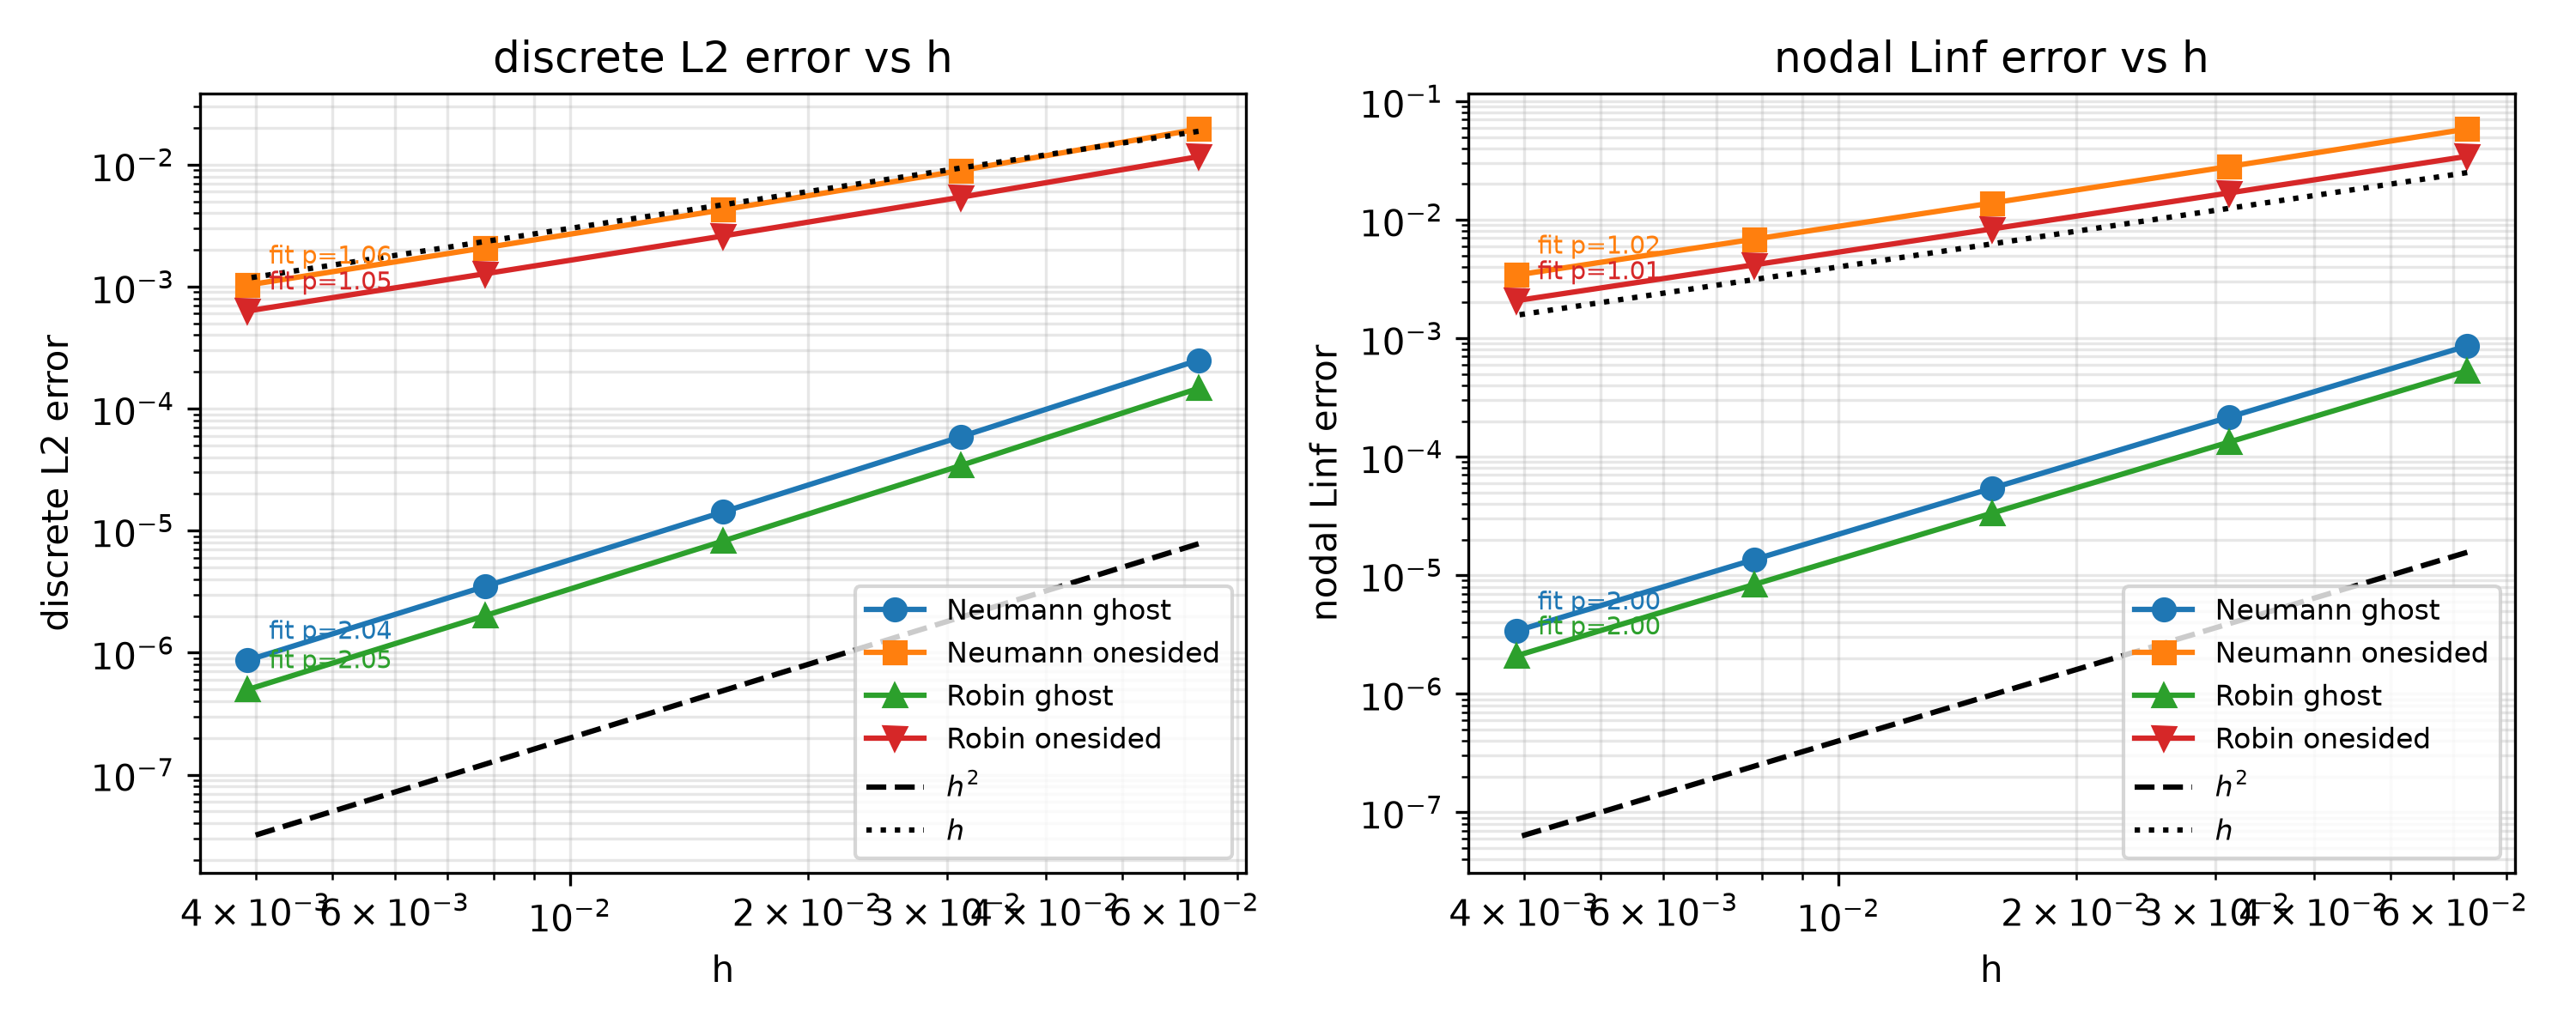
\includegraphics[width=\linewidth]{../figures/fig03c_convergence.png}
\end{columns}

\bigskip
\textbf{Takeaway:} orders match pre-registered expectations --- and the
pairwise rates drift to the fitted ones only on fine grids (documented,
not hidden).
\end{frame}

% ------------------------------------------------------------------
\begin{frame}{Verification 3: falsification --- can we catch a wrong code?}
Three deliberate defects injected into the assembly (exp\_07):

\bigskip
\begin{table}[H]\centering\small
\begin{tabular}{lccc}
\toprule
Run & fitted $p_{h\ell^2}$ & fitted $p_\infty$ & $\lVert e\rVert_\infty$ at $N{=}128$ \\
\midrule
Baseline (correct ghost) & 2.052 & 1.997 & $1.35\times10^{-5}$ \\
F1: sign of $q$ flipped & 0.038 & $-0.002$ & $3.48$ \\
F2: west coupling not doubled & $-0.076$ & $-0.175$ & $6.32$ \\
F3: top-edge Dirichlet move dropped & 0.040 & 0.000 & $7.39$ \\
\bottomrule
\end{tabular}
\end{table}

\textbf{Takeaway:} the refinement study is not decoration --- each defect
destroys the order table in a distinct way. Our tables would have failed.
\end{frame}

% ------------------------------------------------------------------
\begin{frame}{Matrix structure tells the same story}
\begin{columns}
\column{0.5\textwidth}
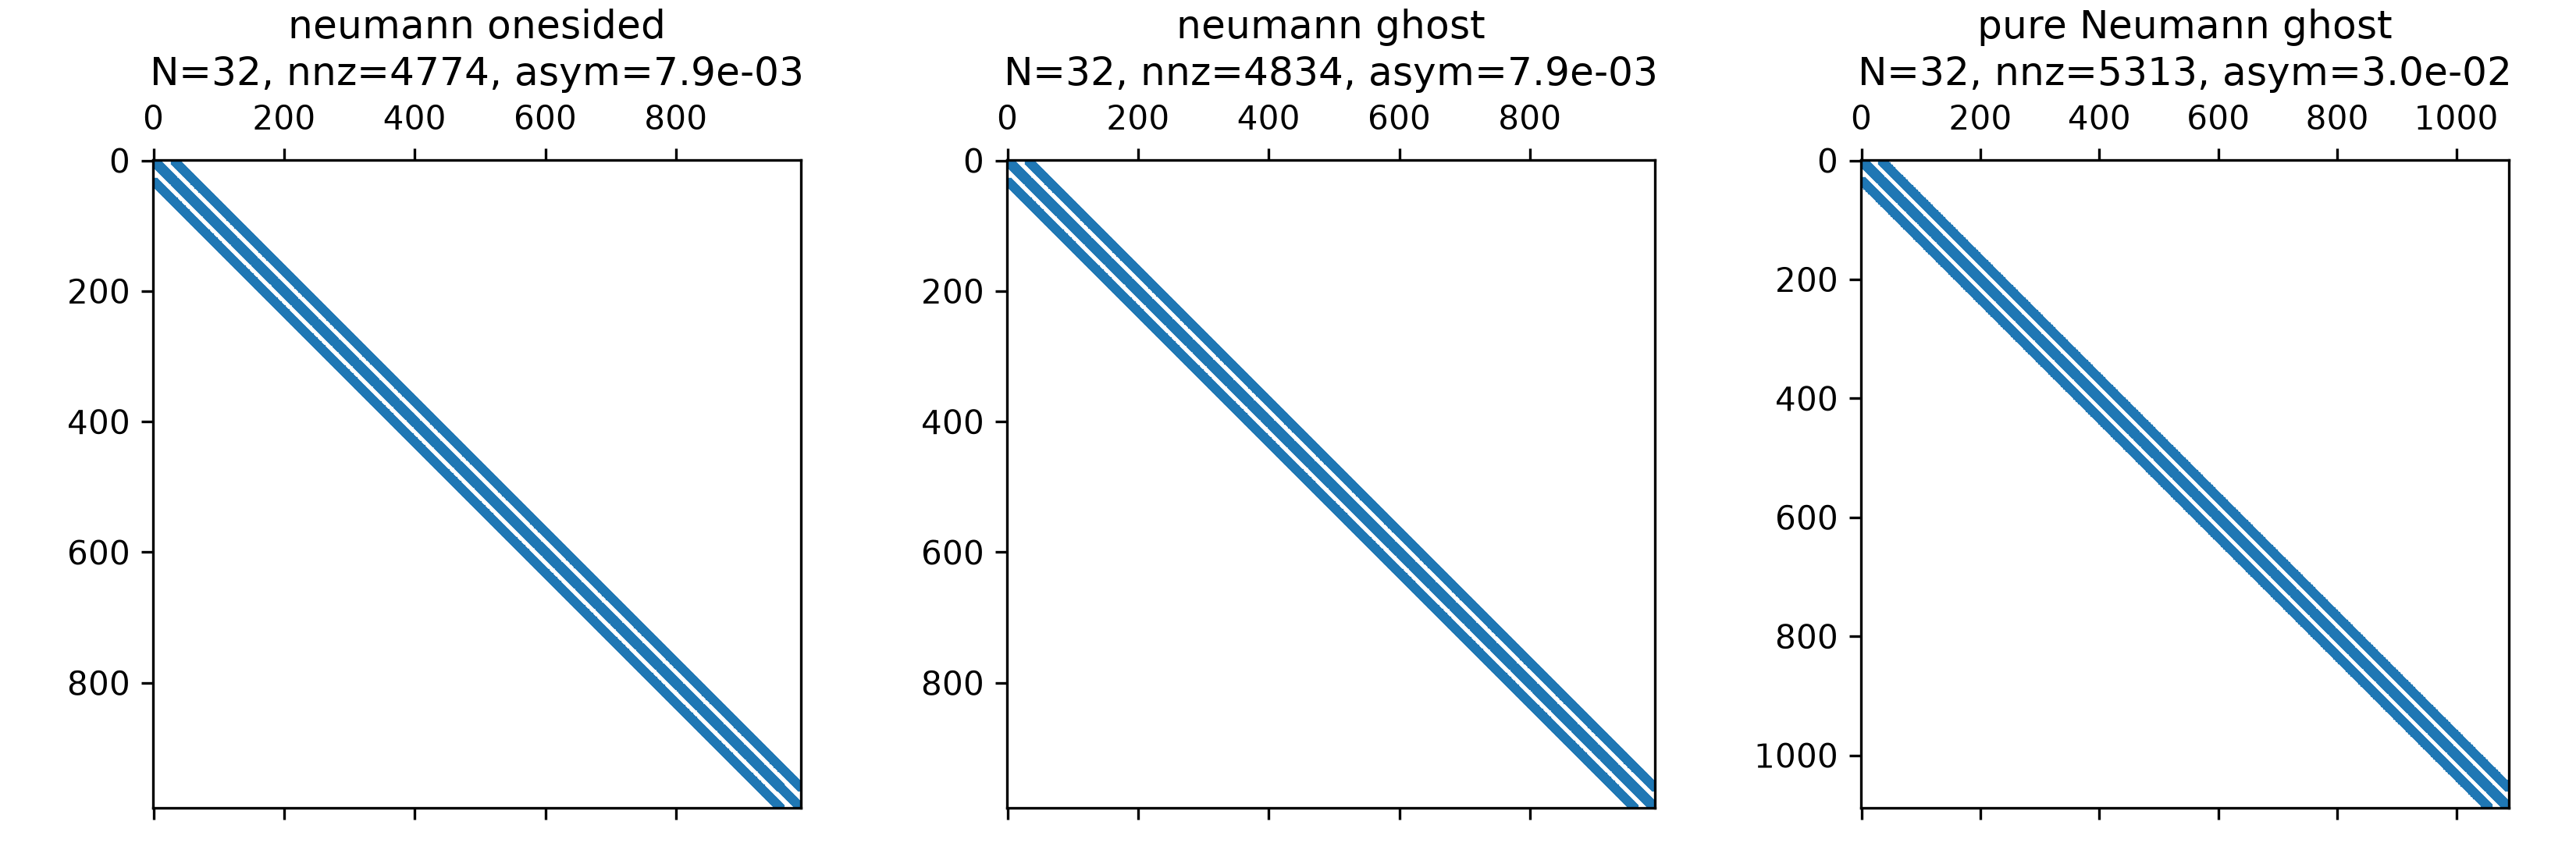
\includegraphics[width=\linewidth]{../figures/fig04_spy.png}

\column{0.46\textwidth}
\begin{itemize}
\item Five-point sparsity everywhere; the closure only changes one
      boundary block.
\item $\norm{A-A^{T}}/\norm{A}$: ghost closure $\approx 0.02$,
      one-sided $\approx 0.15$ --- both nonsymmetric, one-sided worse.
\item Condition number $\kappa \sim C h^{-2}$; the one-sided variant
      has the larger $C$ (M3 predicted this).
\end{itemize}
\end{columns}

\bigskip
\textbf{Takeaway:} structure and conditioning confirm what the errors
say --- no hidden story.
\end{frame}

% ------------------------------------------------------------------
\begin{frame}{Experiments: cost vs.\ accuracy}
\begin{columns}
\column{0.52\textwidth}
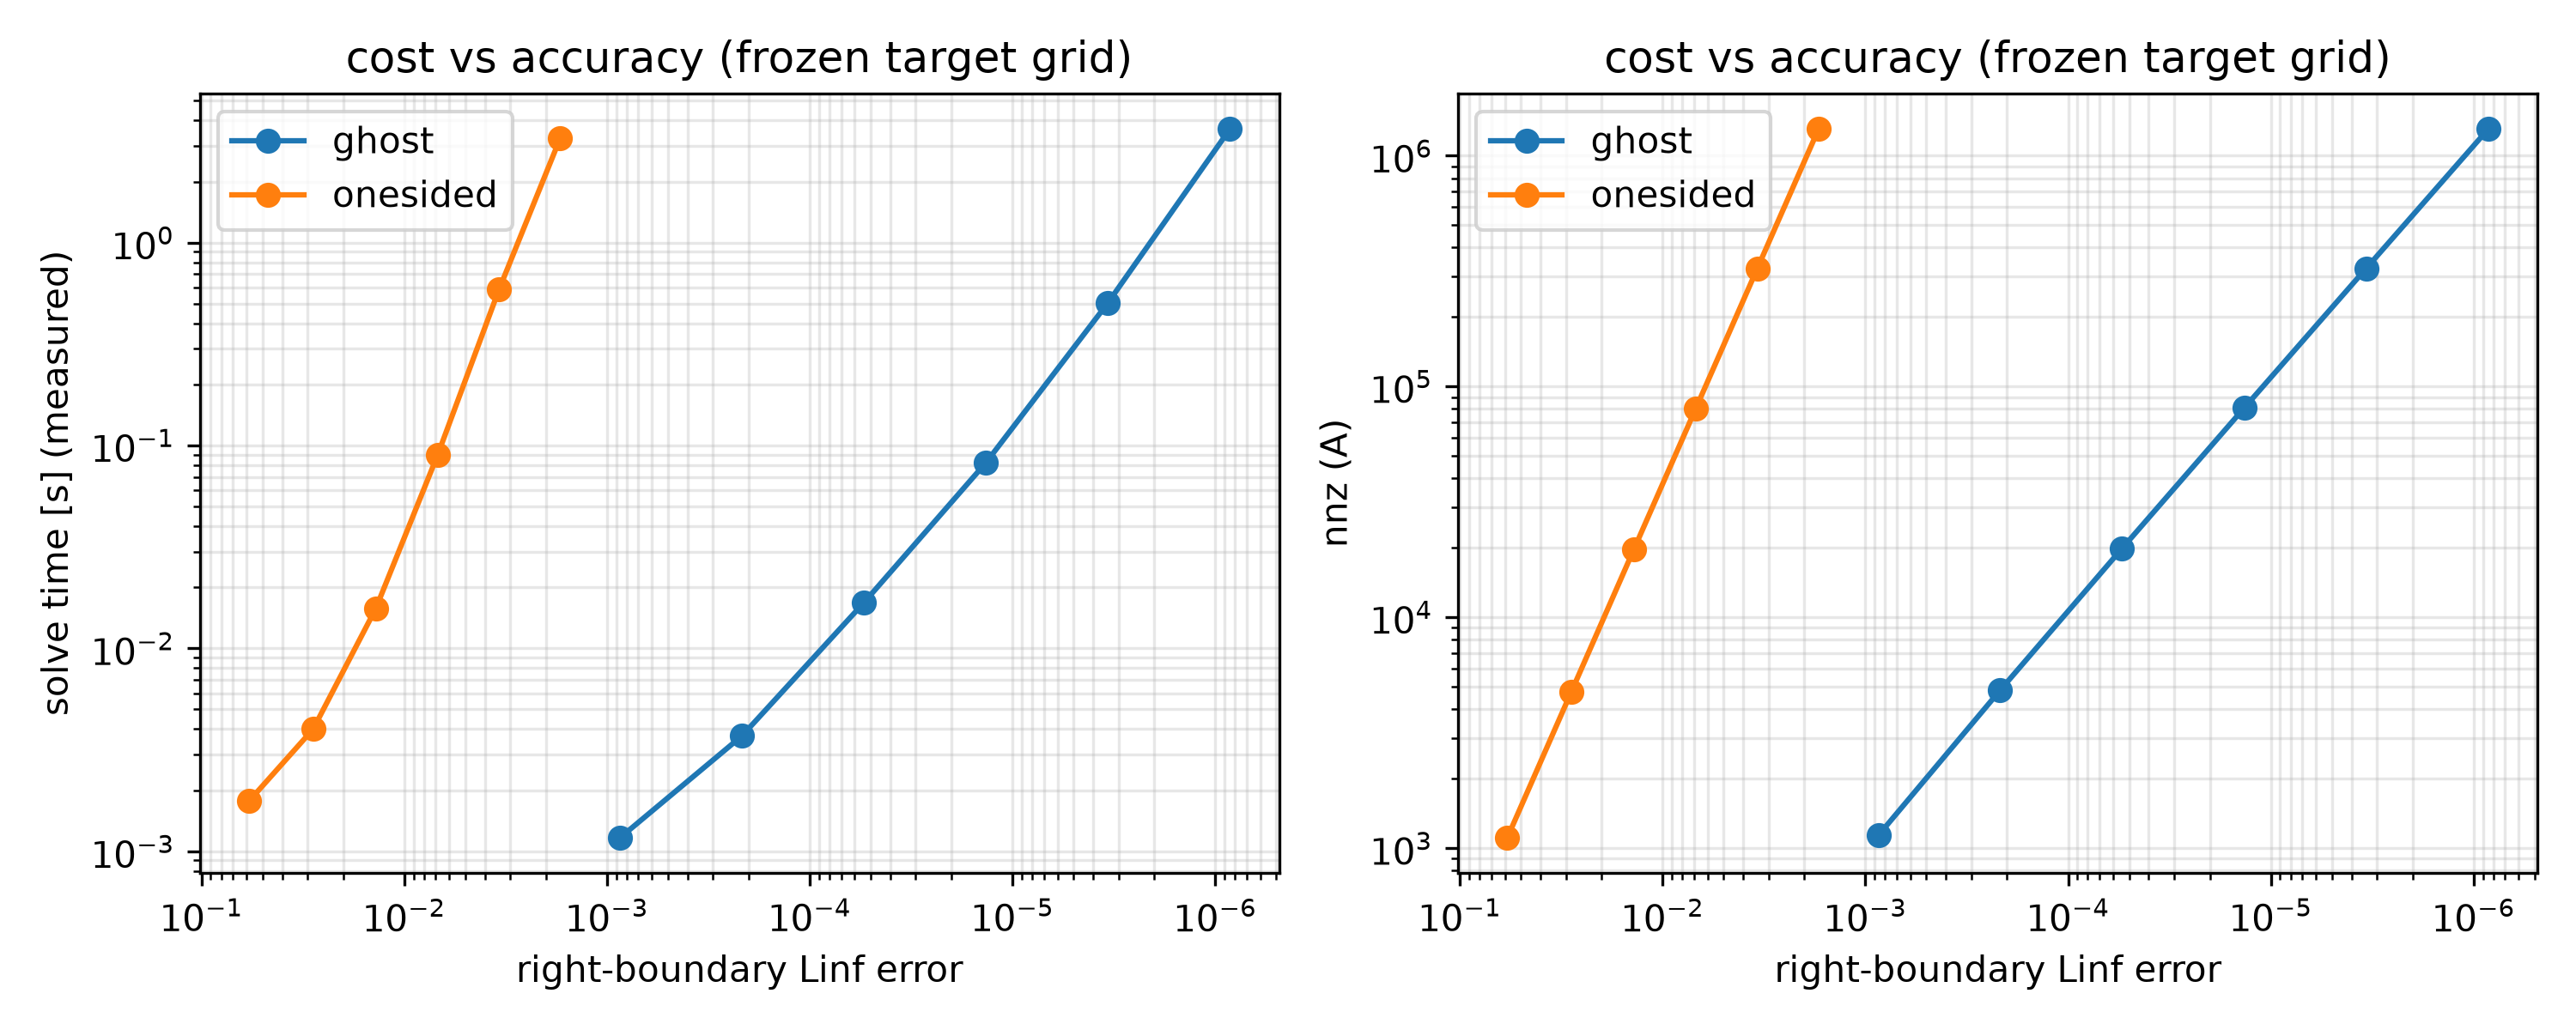
\includegraphics[width=\linewidth]{../figures/fig05_cost_accuracy.png}

\column{0.44\textwidth}
Frozen target $\norm{e}_{\infty,\partial}\le 10^{-4}$:
\begin{itemize}
\item Ghost: $N\approx 47$ ($n\approx 2.2\times10^{3}$) --- cheap.
\item One-sided: $N\approx 8.6\times10^{3}$
      ($n\sim 7\times10^{7}$) --- infeasible for sparse direct.
\end{itemize}
At $N=512$ (same wall time): ghost error $8.5\times10^{-7}$;
one-sided $1.7\times10^{-3}$.
\end{columns}

\bigskip
\textbf{Takeaway:} closure choice is a \alert{feasibility} choice, not
a cosmetic one.
\end{frame}

% ------------------------------------------------------------------
\begin{frame}{Solvers: direct vs.\ iterative}
Matched algebraic accuracy, Neumann/ghost system at $N=64$ ($n=4033$):
\begin{table}[H]\centering\small
\begin{tabular}{lcccc}
\toprule
Solver & Iterations & Time (s) & Rel.\ residual & $\lVert u-u_{\mathrm{splu}}\rVert_\infty$ \\
\midrule
Sparse LU (splu) & 1 factorisation & 0.016 & $1.5\times10^{-15}$ & $0$ \\
BiCGSTAB + ILU & 39 & 0.089 & $8.6\times10^{-11}$ & $6.9\times10^{-9}$ \\
SOR ($\omega=1.5$) & 3721 & 1.664 & $1.0\times10^{-10}$ & $2.5\times10^{-7}$ \\
Gauss--Seidel & 11192 & 4.646 & $1.0\times10^{-10}$ & $2.5\times10^{-7}$ \\
Jacobi & 22388 & 1.979 & $1.0\times10^{-10}$ & $2.5\times10^{-7}$ \\
\bottomrule
\end{tabular}
\end{table}

Tolerance strategy from Week 7: $\mathrm{tol}\sim C h^{2}$ so algebraic
error never pollutes discretisation error.

\textbf{Takeaway:} iterative solvers match direct accuracy at lower
memory; the closure comparison is independent of the solver choice.
\end{frame}

% ------------------------------------------------------------------
\begin{frame}{Depth item: pure-Neumann null space}
Neumann on the \emph{whole} boundary $\Rightarrow$ $A\bm{1}=0$ exactly
(machine zero), smallest left singular vector $=$ constant
($2.6\times10^{-12}$).

\bigskip
\textbf{Discrete compatibility:} $|\langle b,w\rangle|/(\norm{b}\norm{w})
= 5.8\times10^{-6}$ --- not machine zero: corner rows sample two
one-sided data and the trapezoid boundary rule. We report it, not hide it.

\bigskip
Pinned gauge $u(0,0)=0$ + least-squares constant shift:
$L^{2}$ order $2.05$, $L^{\infty}$ order $1.84$
(corners limit the max-norm rate --- bounded, not derived).

\textbf{Takeaway:} the null space is structural, and the recovery is
verifiable; an incompatible RHS is caught by the falsification variant.
\end{frame}

% ------------------------------------------------------------------
\begin{frame}{Conclusions and limitations}
\textbf{Conclusions}
\begin{enumerate}
\item Two second-order-accurate-looking closures give global orders
      $2$ vs.\ $1$ --- the boundary row \emph{is} the method.
\item Ghost elimination buys feasibility: $10^{4}$-fold fewer unknowns
      for the same boundary accuracy.
\item The evidence chain (row defects $\rightarrow$ refinement tables
      $\rightarrow$ falsification $\rightarrow$ structure/cost) makes
      every number auditable; one command
      (\texttt{python run\_all.py}) reproduces all of them.
\end{enumerate}

\bigskip
\textbf{Limitations / open}
\begin{itemize}
\item Square domain only; corners at non-right angles not treated.
\item Pure-Neumann $L^{\infty}$ order $1.84$: attributed to corner
      quadrature, full derivation open.
\item SOR parameter $\omega$ not tuned; AMG comparison is future work.
\end{itemize}
\end{frame}

% ------------------------------------------------------------------
\begin{frame}{Reproducibility \& contributions}
\textbf{One command:} \texttt{python run\_all.py} $\rightarrow$ all
tables, figures, \texttt{results.json}.

\bigskip
\textbf{Team O contributions} (git-traceable):
\begin{itemize}
\item \textbf{Zihan Xu (2360751):} project management, visualisation,
      report \& slides, cost--accuracy study.
\item \textbf{Beixue Liang (2359957):} hand derivations of both closure
      rows, Taylor defects, pure-Neumann solvability, falsification
      design.
\item \textbf{Yumo Li (2253567):} solver implementation and assembly
      code, iterative-solver comparison, unit tests.
\end{itemize}

\bigskip
\centering\Large Thank you --- questions welcome.
\end{frame}

\end{document}
